\chapter{Analisis dan Perancangan}
Pada bab ini dituliskan analisis terkait kebutuhan sistem pada KodeBareng, masalah pada implementasi ILE yang sudah ada, serta rancangan solusi yang akan diimplementasikan.

\section{Analisis Masalah}
%  [\hl{TODO: ANALISIS PERMASALAHAN DIKAITKAN DENGAN PERMASALAHAN PADA PEMROGRAMAN PEMULA. JELASIN JUGA KENAPA BUTUH PEMBELAJARAN INTERKATIF}]

%  [\hl{TODO: JELASIN JUGA PERMASALAHAN PADA PLATFORM2 YANG ADA, BAIK KELAS PEMROGRAMAN MAUPUN PYTHONTUTOR DSB}]

Kompleksitas dari pemrograman itu sendiri menyebabkan sulitnya pelajar yang baru mempelajari pemrograman memahami konsep-konsep dan abstrak dari pemrograman \parencite{moons2013pilot}. Kurangnya kemampuan dalam menelusuri jejak suatu kode program, serta belum terbentuknya model kerangka pikir terhadap cara program komputer bekerja \parencite{mayer1981psychology} merupakan faktor-faktor yang membuat pelajar tidak dapat menyerap informasi teknis baru terkait pemrograman dengan maksimal. Maka dari itu, diperlukan suatu bentuk model konkret terkait alur proses kerja suatu program komputer sehingga dapat mempermudah proses transfer ilmu konsep-konsep pemrograman kepada pelajar. Pembelajaran interaktif menjadi salah satu cara yang dapat dimanfaatkan karena dapat diaplikasikan secara daring menggunakan teknologi digital yang sudah tersedia.

Menurut \textcite{moons2013pilot}, terdapat 4 pendekatan yang dapat dilakukan untuk memecahkan masalah tersebut. Pendekatan pertama adalah dengan menggunakan urutan paradigma pemrograman tertentu dalam pembelajarannya sehingga konsep-konsep yang lebih dalam pada pemrograman tidak harus dipelajari dari awal. Pendekatan kedua adalah dengan menggunakan teknik pembelajaran secara aktif, seperti lokakarya dan penceritaan dengan narasi. Namun, pendekatan ini agak sulit diaplikasikan pada pembelajaran secara daring. Pendekatan ketiga adalah dengan menggunakan bahasa pemrograman yang lebih sesuai untuk pelajar pemrograman, seperti Python dan Eiffel. Pendekatan keempat adalah menggunakan lingkungan pembelajaran interaktif atau \textit{interactive learning environment} (ILE) yang dapat berbentuk \textit{microworld}, visualisasi algoritma, dan visualisasi eksekusi program.

% KodeBareng adalah platform berbasis web sebagai sarana pembelajaran pemrograman menggunakan gamifikasi. Pada platform ini, dibutuhkan suatu \textit{interactive learning environment} (ILE) yang dapat mendukung aktivitas pemrograman secara praktis. ILE diharapkan dapat meningkatkan kemampuan pemecahan masalah dan implementasi kode penggunanya dengan adanya wadah menulis dan menjalankan kode secara daring. ILE dibangun secara modular pada platform KodeBareng sehingga tidak terlalu disruptif terhadap sistem yang sudah ada.

% Dalam beberapa sistem yang sudah ada seperti \href{https://olympia.id/}{Olympia}, ILE yang dapat menjawab kebutuhan ini biasanya berupa sistem submisi kode implementasi yang menggunakan autograder untuk penilaiannya. Sayangnya, hal ini dinilai kurang interaktif karena setiap perubahan kode yang dilakukan pengguna harus melakukan submisi ulang dan menjalankan kembali programnya. Pengguna juga menjadi tidak tahu kesalahannya dimana, serta masih harus dapat menjalankan kodenya secara manual di mesinnya.

% Pada beberapa platform lain seperti yang sudah dibahas pada bab sebelumnya, terdapat berbagai macam jenis ILE yang masing-masing memiliki kelebihan dan kekurangannya masing-masing. ILE visual seperti yang digunakan pada \textcite{brilliant2021media} memiliki interaktivitas yang sangat tinggi dan mudah dipahami, namun kurang dapat diimplementasikan secara umum dan tidak langsung menyentuh implementasi kode. Sementara itu, terdapat juga ILE yang berupa Web IDE namun kebanyakan implementasinya hanya sebatas eksekusi kode pada wadah teks yang diberikan. Keterbatasan ini membuat proses pembelajaran terhambat akibat kurangnya ada pembantu yang dapat digunakan oleh pengguna untuk mencari letak kesalahan dalam implementasi kodenya, serta menjadikan Web IDE terlalu menantang bagi pemula yang ingin belajar pemrograman.

Berdasarkan studi literatur terhadap beberapa platform kelas pembelajaran lainnya, metode pembelajaran pemrograman interaktif secara daring dapat dikategorikan menjadi visual dan non-visual. Metode pembelajaran pemrograman yang visual tidak langsung menggunakan kode seperti pada \textcite{brilliant2021media}, tetapi menggunakan perumpaan visual yang interaktif dengan memakai gambar, simbol, serta animasi. Metode ini membuat pembelajaran menjadi lebih menarik dan mudah, karena diekspresikan dalam bentuk visual sehingga dapat membentuk model kerangka pikir pelajar. Namun, metode ini tidak menyentuh secara langsung aktivitas pemrograman secara praktis sehingga ada kemungkinan dapat terjadi perbedaan antara teori dan praktik yang dipahami pelajar dengan implementasi program yang sebenarnya. Metode ini juga memiliki bentuk yang spesifik terhadap konten materi yang dibawa, sehingga tidak dapat dipakai untuk konten materi lainnya. \textcite{froggy2021media} juga termasuk pada kategori ini, karena implementasinya hanya spesifik pada materi yang dibawa, khususnya pada materi pengembangan web.

Metode non-visual mayoritas menggunakan Web IDE dalam pembelajarannya. Pengguna dapat berinteraksi dengan Web IDE sehingga mereka dapat melatih kemampuan pemecahan masalah dan pemrograman praktis. Web IDE yang digunakan biasanya memiliki kapabilitas untuk mengembalikan hasil keluaran dari eksekusi kode, serta melakukan penilaian terhadap kebenaran implementasi. Web IDE juga dapat menerima berbagai macam bahasa sesuai dengan kebutuhan materi yang sedang dipelajari. Selain itu, terdapat juga Web IDE yang menyimulasikan terminal ketimbang editor kode seperti yang dapat dilihat di Katacoda \parencite{katacoda2021media}. Terdapat juga platform seperti \textcite{progate2021media} yang memanfaatkan pembelajaran interaktif dengan pendekatan "melalui" penyampaian materi secara visual dan naratif. Namun, kebanyakan dari implementasi metode ini hanya berfokus pada aspek latihan pemrograman praktis saja, tidak memerhatikan permasalahan terhadap pelajar yang telah dibahas sebelumnya.

Diluar dari platform-platform kelas pembelajaran pemrograman, sebenarnya terdapat berbagai macam pembelajaran interaktif yang menawarkan solusi yang lebih variatif, seperti pada \textcite{tran2013interactive} IDE yang dibuat digabungkan dengan aspek interaktif berupa kolaborasi antara pelajar dengan pelajar lainnya. Terdapat juga implementasi pada \textcite{guo2013pythontutor} serta \textcite{moons2013pilot} yang menerapkan pendekatan keempat berupa visualisasi eksekusi kode. Visualisasi eksekusi kode menjadi salah satu aspek yang menarik karena tidak banyak ditemukan implementasinya pada platform kelas pembelajaran pemrograman yang sudah ada. Hal ini akan menjadi keunikan tersendiri karena berbeda dari platform kelas pembelajaran pemrograman lainnya sehingga dapat menjadi nilai tambah pada platform pembelajaran pemrograman KodeBareng.

% [\hl{TODO: MASUKIN ANALISIS BISNIS MULTIDIMENSIONAL DISINI}]

% Selain itu, Web IDE bisa dikembangkan lebih lanjut pada aspek kolaboratif \parencite{tran2013interactive} ataupun mendukung visualisasi langkah eksekusi program seperti pada \textcite{guo2013pythontutor}. Visualisasi langkah eksekusi menjadi salah satu aspek yang menarik karena tidak banyak ditemukan implementasinya pada platform pembelajaran pemrograman yang sudah terkenal.

% REVISI II
% KodeBareng adalah platform berbasis web sebagai sarana pembelajaran pemrograman menggunakan gamifikasi. Metode pembelajarannya berbasis teks, visual interaktif, serta kuis-kuis. Kuis-kuis tersebut dapat berupa pilihan ganda, isian singkat, ataupun pencocokan jawaban yang membahas materi terkait yang sudah dipelajari. Dengan adanya kuis tersebut, diharapkan pelajar tidak hanya bisa memahami teori namun juga implementasi kode dari teori yang telah dijabarkan, seperti dengan adanya pertanyaan terkait hasil keluaran suatu kode. Namun, pertanyaan kuis semacam itu memiliki limitasi karena pelajar tidak dapat membuat sendiri implementasi kode sehingga susah untuk mengukur pemahaman praktis dan kemampuan pemecahan masalah menggunakan teori yang telah diberikan. Padahal, pemrograman adalah suatu kemampuan yang membutuhkan banyak latihan praktik implementasi agar pemahaman dapat tercapai secara optimal.

% Alternatif lain juga bisa dengan memberikan permasalahan yang harus dipecahkan kemudian pelajar dapat mengimplementasikan sendiri terlebih dahulu di mesinnya lalu melakukan submisi kode pada platform. Hal ini menimbulkan permasalahan lain seperti susahnya melakukan pemecahan permasalahan pada instalasi spesifik mesin yang digunakan oleh pelajar, adanya perbedaan versi dari lingkungan mesin pelajar dan mesin penguji yang dapat menimbulkan masalah dalam pengetesan, dan juga membuat platform lebih terbatas portabilitasnya karena instalasi hanya terbatas pada mesin dan lingkungan sistem tertentu. Permasalahan lain juga timbul dari cara melakukan penilaian dan pengetesan kode yang telah dibuat, karena apabila dilakukan secara manual akan membutuhkan banyak tenaga kerja.

% REVISI I
% Saat ini, terdapat banyak sekali metode penyampaian materi pembelajaran pemrograman secara daring. Namun, agar dapat memvalidasi pengetahuan yang didapat diperlukan sistem pendukung yang dapat digunakan sebagai media praktik bagi para pelajar. Kurangnya praktik dan latihan dalam pembelajaran dapat membuat adanya pemisah antara pemahaman teori dan praktik. (\textit{!TODO: ceritakan paper mengenai ini})

% Untuk memvalidasi pengetahuan yang sudah dipelajari, terdapat banyak metode yang dapat digunakan. Salah satu metode yang sering dipakai adalah kuis yaitu serangkaian pertanyaan yang mengacu pada materi yang telah diberikan. Kuis dapat dibuat dalam berbagai macam bentuk seperti pilihan ganda, isian singkat, esai, dll. Metode esai dapat digunakan untuk memvalidasi logika dan pola pikir dari pemecahan masalah, namun karena esai tersebut merupakan kode maka harus terdapat sistem yang dapat mengeksekusi, menilai, serta memberikan \textit{feedback} dari hasil eksekusi kode tersebut layaknya pemrograman yang sebenarnya.

% Maka dari itu, diperlukan sistem pembelajaran pemrograman interaktif yang dapat dipakai pengguna untuk menuliskan kode, memberikan \textit{feedback} dari kode yang dibuat, serta menilai kebenaran dari kode tersebut. \textit{Feedback} yang diberikan berupa hasil eksekusi kode berupa pesan keluaran apabila kode berhasil dijalankan, serta pesan error apabila terjadi masalah dalam eksekusi kode. Pesan keluaran hasil eksekusi dapat dibandingkan dengan pesan keluaran yang seharusnya agar dapat dinilai dan diberitahukan kepada pengguna sehingga pengguna dapat mengetahui letak kesalahan dari kode yang diimplementasikan.

\section{Analisis Kebutuhan} \label{sec:analisis-kebutuhan}
Seperti yang sudah dijelaskan pada Bab sebelumnya, KodeBareng merupakan platform web pembelajaran pemrograman yang ingin membawakan pembelajarannya secara visual dan interaktif. Berdasarkan analisis masalah, pendekatan yang akan dipilih adalah dengan membuat ILE berupa visualisasi eksekusi kode yang akan diintegrasikan pada platform web KodeBareng. ILE tesebut dapat memvisualisasikan eksekusi kode yang diberikan sehingga dapat memberikan gambaran mengenai bagaimana alur cara suatu kode program bekerja. Berbeda dengan platform lainnya yang mendukung interaktivitasnya dengan adanya animasi visual ataupun Web IDE yang dapat mengeksekusi program secara langsung, pendekatan dengan menggunakan visualisasi eksekusi kode dapat diintegrasikan dengan pembawaan materi pembelajaran serta pengerjaan latihan soal sehingga dapat mencapai tujuannya yaitu meningkatkan pemahaman orang yang baru mempelajari pemrograman dengan memberikan model kerangka eksekusi kode yang dapat dieksplorasi menggunakan kodenya sendiri. Pendekatan ini sesuai dengan yang dilakukan oleh \textcite{moons2013pilot} dan \textcite{mayer1981psychology}.

Maka dari itu, dibuatlah diagram \textit{use case} baru yang sesuai dengan kebutuhan dan pendekatan terkait yang dapat dilihat pada \autoref{fig:diagram-usecase-v2}. Penjelasan terkait \textit{use case} tersebut dapat dilihat pada \autoref{tab:exp-diagram-usecase-v2}.

\begin{figure}[H]
  \centering
  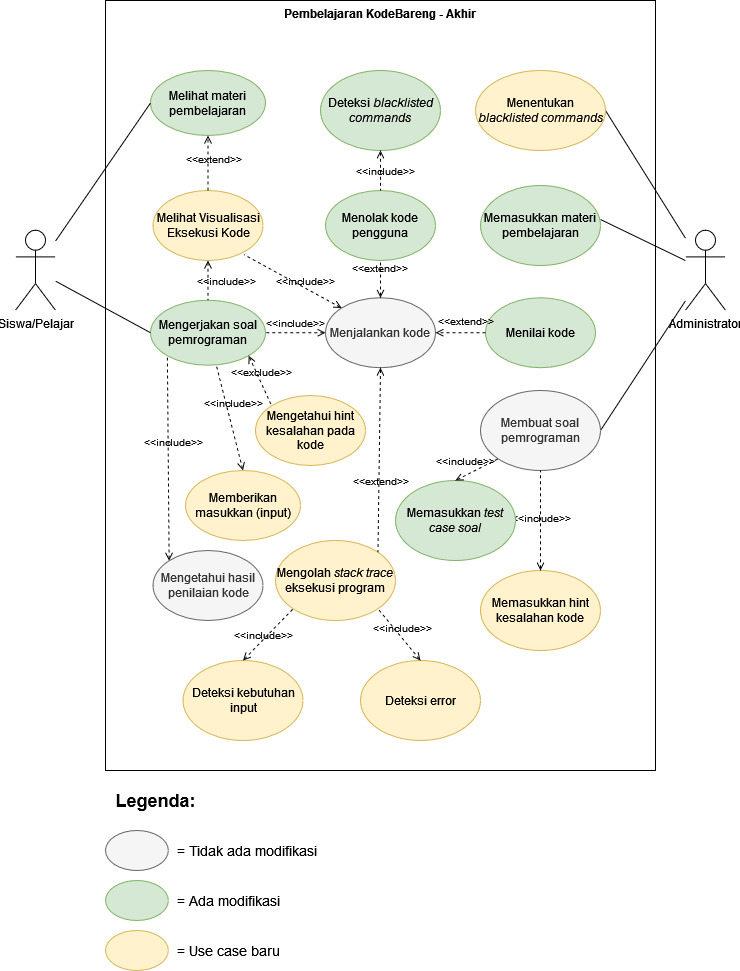
\includegraphics[width=1.15\textwidth]{chapter3/diagram_usecase_v2.jpg}
  \caption{\textit{Use Case} pembelajaran pemrograman KodeBareng setelah perubahan \\ Sumber: Penulis (2022)} \label{fig:diagram-usecase-v2}
\end{figure}

\small
\begin{longtable}[c]{|l|>{\setlength{\baselineskip}{0.75\baselineskip}}p{0.3\linewidth}|>{\setlength{\baselineskip}{0.75\baselineskip}}p{0.5\linewidth}|}
  \caption{Penjelasan \textit{Use Case} pembelajaran pemrograman KodeBareng setelah perubahan} \label{tab:exp-diagram-usecase-v2}                                                                                                                                                                                                                     \\ \hline
  \rowcolor{gray!30}
  \textbf{ID} & \textbf{Kebutuhan}                             & \textbf{Penjelasan}                                                                                                                                                                                                                                                                  \\ \hline
  \endfirsthead
  %
  \caption*{\autoref{tab:exp-diagram-usecase-v2} (lanjutan): Penjelasan \textit{Use Case} pembelajaran pemrograman KodeBareng setelah perubahan}                                                                                                                                                                                                      \\ \hline
  \rowcolor{gray!30}
  \textbf{ID} & \textbf{Kebutuhan}                             & \textbf{Penjelasan}                                                                                                                                                                                                                                                                  \\ \hline
  \endhead
  %
  UC-01       & Melihat materi pembelajaran                    & Pengguna dapat melihat materi pembelajaran berupa teks dan gambar. Perubahannya adalah integrasi ILE  sehingga pada materi dapat dimasukkan visualisasi eksekusi kode.                                                                                                               \\ \hline
  UC-02       & Mengerjakan soal pemrograman                   & Pengguna dapat mengerjakan latihan soal pemrograman. Perubahannya adalah soal pemrograman kini dilengkapi ILE yang dapat memvisualisasikan eksekusi kode serta memberikan hint apabila ada kesalahan dalam mengerjakan soal.                                                         \\ \hline
  UC-03       & Melihat visualisasi eksekusi kode              & Pengguna dapat melihat visualisasi kode berupa alur kerja eksekusi program serta data-data apa saja yang terdapat dalam memori.                                                                                                                                                      \\ \hline
  UC-04       & Mengetahui hasil penilaian kode                & Pengguna dapat mengetahui kebenaran dari kode yang dimasukkan pada latihan pemrograman.                                                                                                                                                                                              \\ \hline
  UC-05       & Memberikan masukkan (input)                    & Pengguna dapat memberikan input yang akan dimasukkan pada kode yang akan dieksekusi.                                                                                                                                                                                                 \\ \hline
  UC-06       & Mengetahui hint kesalahan pada kode            & Pengguna dapat melihat hint kesalahan apabila kode yang dimasukkan pada latihan pemrograman salah.                                                                                                                                                                                   \\ \hline
  UC-07       & Menjalankan kode                               & Pengguna dapat menjalankan kode yang dimasukkan serta melihat keluarannya.                                                                                                                                                                                                           \\ \hline
  UC-08       & Menolak kode pengguna                          & Kode yang dimasukkan oleh pengguna dapat ditolak oleh sistem apabila tidak sesuai dengan batasan-batasan perintah yang dapat dieksekusi oleh ILE. Perubahannya adalah batasan eksekusi program dapat ditentukan oleh administrator (sebelumnya ditentukan secara \textit{hard code}) \\ \hline
  UC-09       & Deteksi \textit{blacklisted commands}          & Sistem memiliki daftar perintah yang tidak boleh dieksekusi agar tidak mengancam keamanan sistem. Perubahannya adalah perintah yang dieksekusi kini bersifat dinamis tergantung pada definisi yang diberikan oleh Administrator.                                                     \\ \hline
  UC-11       & Menilai kode                                   & Sistem dapat menilai kode yang dijalankan secara \textit{blackbox autograding}. Perubahannya adalah penilaian kini dapat menggunakan lebih dari satu \textit{test case} serta dapat menerima \textit{input}.                                                                         \\ \hline
  UC-12       & Mengolah \textit{stack trace} eksekusi program & Sistem dapat mengolah \textit{stack trace} dari program yang dieksekusi agar dapat memperoleh informasi alur kerja dan data selama eksekusi program.                                                                                                                                 \\ \hline
  UC-13       & Deteksi kebutuhan input                        & Sistem dapat mendeteksi jika kode program membutuhkan input untuk melanjutkan eksekusinya.                                                                                                                                                                                           \\ \hline
  UC-14       & Deteksi error                                  & Sistem dapat mendeteksi error pada eksekusi program.                                                                                                                                                                                                                                 \\ \hline
  UC-15       & Menentukan \textit{blacklisted commands}       & Administrator dapat menentukan perintah-perintah yang tidak boleh dieksekusi pada kode program.                                                                                                                                                                                      \\ \hline
  UC-16       & Memasukkan materi pembelajaran                 & Administrator dapat memasukkan penjelasan materi pada modul-modul kelas pembelajaran. Perubahannya adalah Administrator dapat menambahkan visualisasi eksekusi kode dalam penjelasan materi.                                                                                         \\ \hline
  UC-17       & Membuat soal pemrograman                       & Administrator dapat membuat soal pemrograman.                                                                                                                                                                                                                                        \\ \hline
  UC-18       & Memasukkan \textit{test case} soal             & Administrator dapat memasukkan \textit{test case} penilaian pada suatu soal. Perubahannya adalah \textit{test case} yang dimasukkan bisa lebih dari satu dan memiliki input masing-masing.                                                                                           \\ \hline
  UC-19       & Memasukkan hint kesalahan kode                 & Administrator dapat menentukan hint kesalahan yang ditampilkan pada suatu soal.                                                                                                                                                                                                      \\ \hline
\end{longtable}
\normalsize

Berdasarkan \textit{use case} baru yang telah dibuat pada \autoref{fig:diagram-usecase-v2}, diturunkanlah spesifikasi kebutuhan perangkat lunak fungsional dan non-fungsional yang dapat dilihat pada \autoref{tab:srs-fungsional} dan \autoref{tab:srs-nonfungsional}.

Spesifikasi fungsional menjelaskan fungsi-fungsi yang dapat dijalankan pada ILE yang akan dibuat. Spesifikasi ini diturunkan dari diagram \textit{use case} sesuai dengan siapa dan apa yang dapat dilakukan. Berikut adalah penjelasan lebih detail mengenai spesifikasi fungsional pada \autoref{tab:srs-fungsional}.

\small
\begin{longtable}[c]{|l|>{\setlength{\baselineskip}{0.75\baselineskip}}p{0.5\linewidth}|>{\setlength{\baselineskip}{0.75\baselineskip}}p{0.3\linewidth}|}
  \caption{Spesifikasi kebutuhan fungsional ILE KodeBareng} \label{tab:srs-fungsional}                                                                                                                                                                                    \\ \hline
  \rowcolor{gray!30}
  \textbf{ID} & \textbf{Kebutuhan}                                                                       & \textbf{Penjelasan}                                                                                                                                            \\ \hline
  \endfirsthead
  %
  \caption*{\autoref{tab:srs-fungsional} (lanjutan): Spesifikasi kebutuhan fungsional ILE KodeBareng}                                                                                                                                                                     \\ \hline
  \rowcolor{gray!30}
  \textbf{ID} & \textbf{Kebutuhan}                                                                       & \textbf{Penjelasan}                                                                                                                                            \\ \hline
  \endhead
  %
  KB-F-01     & Pengguna memasukkan kode program pada sistem                                             & Menggunakan kakas Monaco Editor.                                                                                                                               \\ \hline
  KB-F-02     & Pengguna memasukkan input program pada sistem                                            & Masukan diminta apabila kode membutuhkan masukan.                                                                                                              \\ \hline
  KB-F-03     & Pengguna dapat menjalankan kode                                                          & Pengguna dapat melihat hasil eksekusi kode.                                                                                                                    \\ \hline
  KB-F-04     & Pengguna dapat melihat hasil visualisasi eksekusi kode                                   & Pengguna dapat melihat perubahan data dan \textit{flow} program yang dijalankan. Pengguna juga dapat mengeksplorasi langkah-langkah eksekusi.                  \\ \hline
  KB-F-05     & Pengguna mendapat penilaian dari hasil eksekusi kode                                     & Penilaian berdasarkan teknik \textit{blackbox autograding}.                                                                                                    \\ \hline
  KB-F-06     & Pengguna mendapat \textit{hint} kesalahan pada kode program                              & -                                                                                                                                                              \\ \hline
  KB-F-07     & Pengguna dapat melihat pesan error pada program                                          & -                                                                                                                                                              \\ \hline
  KB-F-08     & Sistem menolak kode pengguna apabila terdapat perintah-perintah yang tidak diperbolehkan & Keterbatasan eksekusi ditentukan oleh Administrator.                                                                                                           \\ \hline
  KB-F-09     & Sistem menilai kode program menggunakan \textit{test case}                               & -                                                                                                                                                              \\ \hline
  KB-F-10     & Sistem mengolah \textit{stack trace} eksekusi program                                    & \textit{Stack trace} berisi daftar fungsi, variabel, modul, serta \textit{stack frame} pada tiap langkah eksekusi program. Debugger yang digunakan adalah pdb. \\ \hline
  KB-F-11     & Administrator menentukan perintah-perintah yang tidak diperbolehkan                      & -                                                                                                                                                              \\ \hline
  KB-F-12     & Administrator memasukkan konten materi pembelajaran                                      & Dapat memasukkan visualisasi kode pada materi pembelajaran.                                                                                                    \\ \hline
  KB-F-13     & Administrator membuat soal pemrograman                                                   & -                                                                                                                                                              \\ \hline
  KB-F-14     & Administrator memasukkan \textit{test case} soal pemrograman                             &                                                                                                                                                                \\ \hline
  KB-F-15     & Administrator memasukkan \textit{hint} kesalahan yang dapat ditampilkan pada soal        & -                                                                                                                                                              \\ \hline
\end{longtable}
\normalsize

Spesifikasi non-fungsional diturunkan dari kebutuhan KodeBareng agar tujuan dapat tercapai dan sistem berjalan dengan lancar. Maka dari itu, diturunkanlah spesifikasi berupa batasan respon hasil eksekusi agar pengguna tidak terlalu lama menunggu hasil eksekusi, desain sistem yang memudahkan dilakukan pengetesan terhadap berbagai macam kode, serta membatasi apa yang dapat dieksekusi agar keamanan sistem dapat terjaga. Berikut adalah penjelasan lebih detail mengenai spesifikasi fungsional pada \autoref{tab:srs-nonfungsional}.

\small
\begin{longtable}[c]{|l|l|>{\setlength{\baselineskip}{0.75\baselineskip}}p{0.6\linewidth}|}
  \caption{Spesifikasi kebutuhan non-fungsional ILE KodeBareng} \label{tab:srs-nonfungsional}                \\ \hline
  \rowcolor{gray!30}
  \textbf{ID} & \textbf{Parameter} & \textbf{Kebutuhan}                                                      \\ \hline
  \endfirsthead
  %
  \caption*{\autoref{tab:srs-nonfungsional} (lanjutan): Spesifikasi kebutuhan non-fungsional ILE KodeBareng} \\ \hline
  \rowcolor{gray!30}
  \textbf{ID} & \textbf{Parameter} & \textbf{Kebutuhan}                                                      \\ \hline
  \endhead
  %
  KB-NF-01    & Performance        & Sistem mengembalikan hasil eksekusi paling lama 10 detik.               \\ \hline
  KB-NF-02    & Testability        & Sistem dirancang sedemikian rupa sehingga mudah dilakukan pengetesan.   \\ \hline
  KB-NF-03    & Security           & Sistem tidak membiarkan terjadinya eksekusi kode berbahaya.             \\ \hline
\end{longtable}
\normalsize

Berikut adalah pemetaan hasil penurunan antara \textit{use case} dengan spesifikasi kebutuhan terkait yang dapat dilihat pada \autoref{tab:srs-usecase}.

\small
\begin{longtable}[c]{|l|>{\setlength{\baselineskip}{0.75\baselineskip}}p{0.5\linewidth}|}
  \caption{Keterkaitan SRS dan Use Case} \label{tab:srs-usecase}                \\ \hline
  \rowcolor{gray!30}
  \textbf{ID SRS} & \textbf{ID Use Case}                                        \\ \hline
  \endfirsthead
  %
  \caption*{\autoref{tab:srs-usecase} (lanjutan): Keterkaitan SRS dan Use Case} \\ \hline
  \rowcolor{gray!30}
  \textbf{ID SRS} & \textbf{ID Use Case}                                        \\ \hline
  \endhead
  %
  KB-F-01         & UC-02                                                       \\ \hline
  KB-F-02         & UC-05, UC-13                                                \\ \hline
  KB-F-03         & UC-02, UC-04, UC-07                                         \\ \hline
  KB-F-04         & UC-01, UC-02, UC-03                                         \\ \hline
  KB-F-05         & UC-04, UC-11                                                \\ \hline
  KB-F-06         & UC-06                                                       \\ \hline
  KB-F-07         & UC-02, UC-14                                                \\ \hline
  KB-F-08         & UC-08, UC-09                                                \\ \hline
  KB-F-09         & UC-11                                                       \\ \hline
  KB-F-10         & UC-12                                                       \\ \hline
  KB-F-11         & UC-15                                                       \\ \hline
  KB-F-12         & UC-16                                                       \\ \hline
  KB-F-13         & UC-17                                                       \\ \hline
  KB-F-14         & UC-18                                                       \\ \hline
  KB-F-15         & UC-19                                                       \\ \hline
\end{longtable}
\normalsize

\section{Rancangan Solusi}

Berdasarkan hasil analisis permasalahan dan kebutuhan sebelumnya, dibuatlah rancangan komponen implementasi pada subsistem-subsistem yang terdapat pada KodeBareng. Rancangan tersebut berupa diagram komponen yang terdapat pada \autoref{fig:diagram-komponen}. Rancangan ini menggambarkan komponen apa saja yang akan dimodifikasi ataupun ditambahkan pada sistem KodeBareng terkait pembelajaran pemrograman yang sudah ada.

\begin{figure}[H]
  \centering
  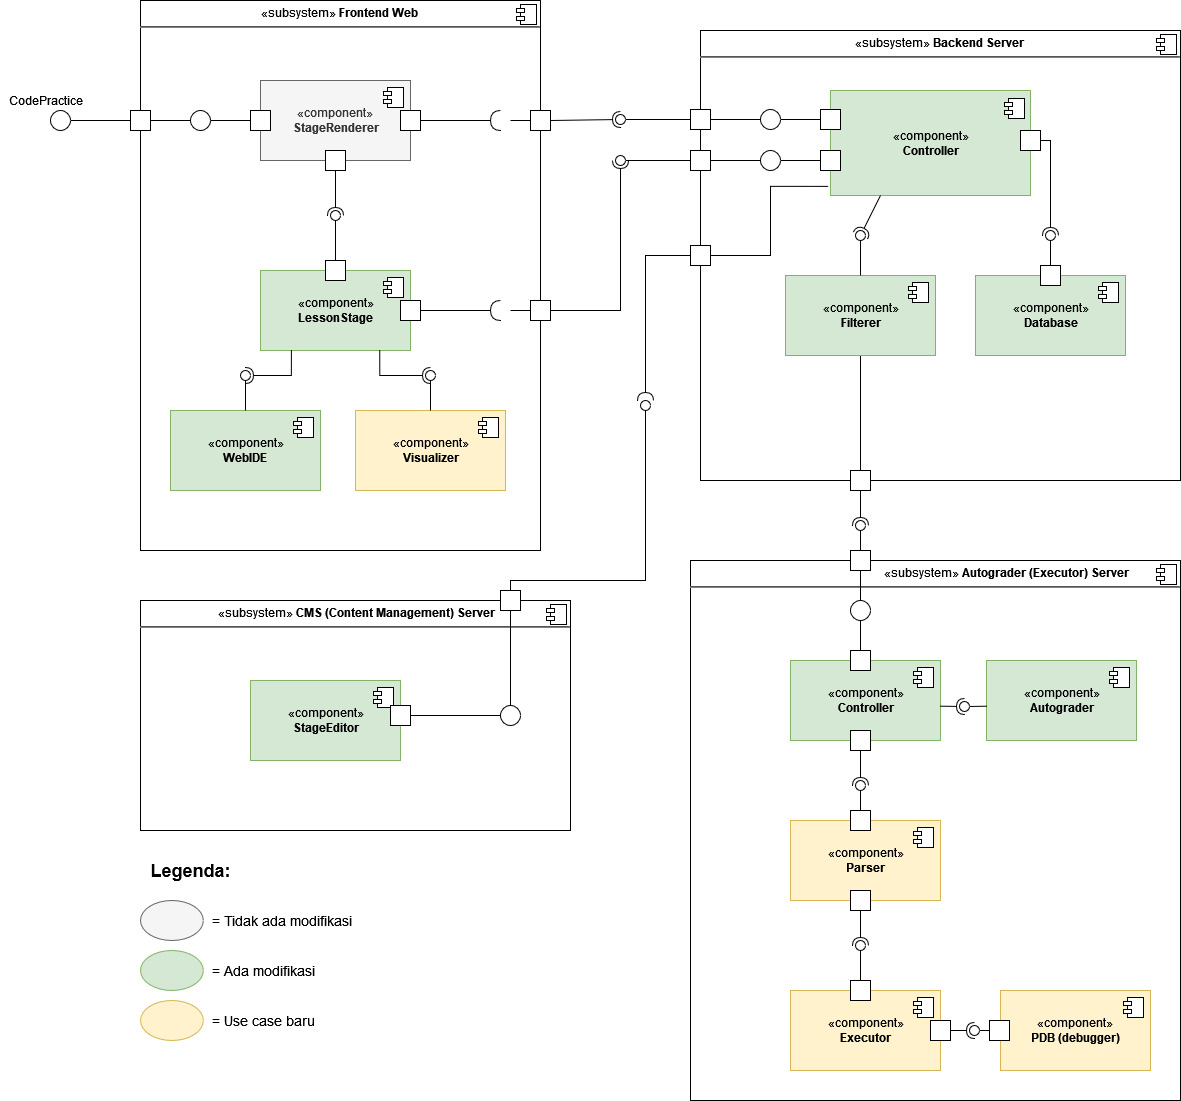
\includegraphics[width=\textwidth]{chapter3/diagram_komponen.jpg}
  \caption{Diagram komponen \\ Sumber: Penulis (2022)} \label{fig:diagram-komponen}
\end{figure}

ILE akan diintegrasikan pada komponen-komponen terkait materi pembelajaran di KodeBareng. Maka dari itu, komponen-komponen yang akan dimodifikasi atau ditambahkan akan terkait dengan komponen Stage yang mendefinisikan bagaimana suatu tahap (\textit{stage}) materi pada suatu modul pembelajaran dijelaskan (berupa teks, latihan pemrograman, dsb). Alur pembelajaran pengguna dapat dilihat pada \autoref{fig:activity-overall}.

\begin{figure}[H]
  \centering
  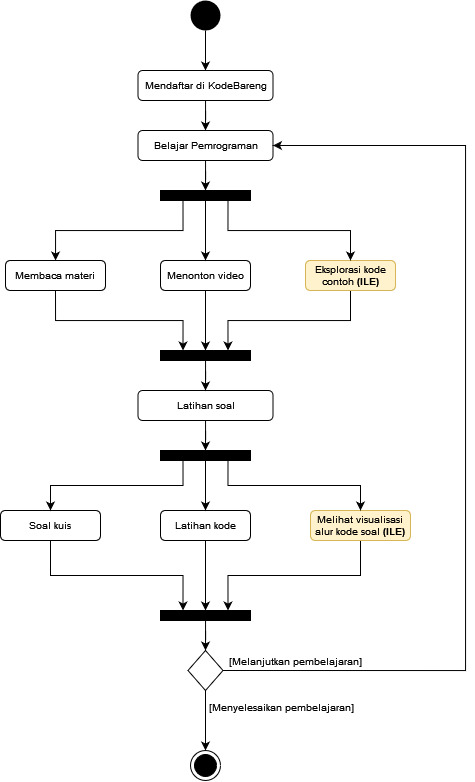
\includegraphics[width=0.85\textwidth]{chapter3/activity-overall.jpg}
  \caption{Activity Diagram Pengguna \\ Sumber: Penulis (2022)} \label{fig:activity-overall}
\end{figure}

Alur program utama terkait visualisasi eksekusi kode dimulai dari pengguna atau sistem memasukkan kode pada Web IDE yang digunakan pada sistem \textit{Frontend}, kemudian melakukan permintaan kepada sistem \textit{Backend} untuk memvisualisasikan kode tersebut. Sistem \textit{Backend} akan memfilter kode yang akan dieksekusi, lalu apabila lolos akan dilanjutkan kepada sistem \textit{Executor} untuk mendapatkan hasil olahan eksekusi program yang dapat divisualisasikan. Hasil tersebut dikembalikan pada sistem \textit{Frontend} untuk divisualisasikan dan dieksplorasi langkah-langkah eksekusinya oleh pengguna. Pada \autoref{fig:activity-ile} dapat dilihat alur program utama ketika dijalankan oleh pengguna.

\begin{figure}[H]
  \centering
  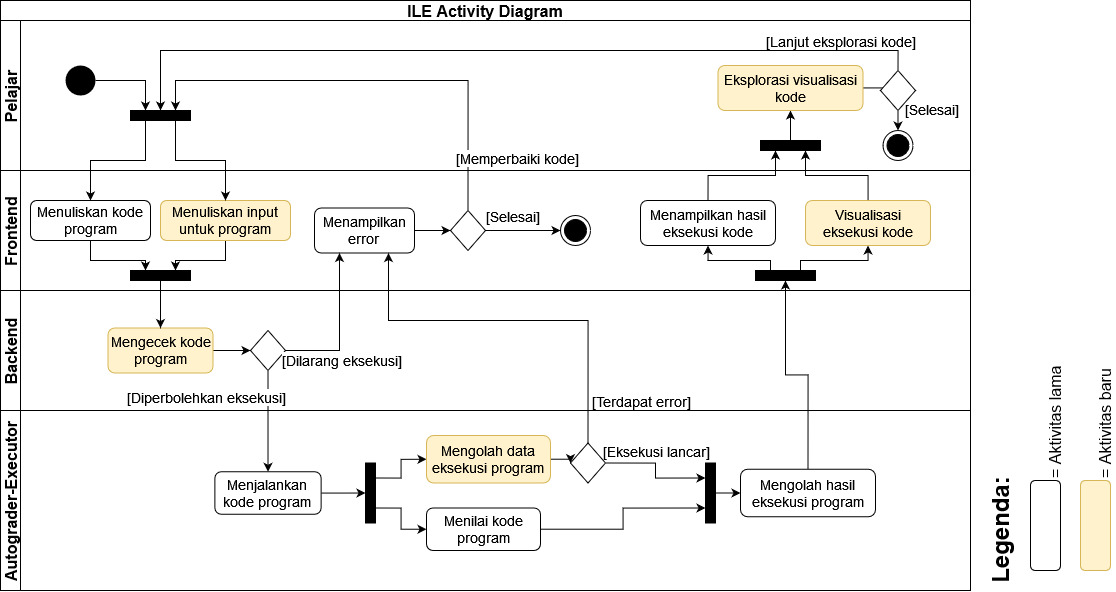
\includegraphics[width=1.8\textwidth, angle=-90]{chapter3/activity-ile.jpg}
  \caption{Activity Diagram ILE \\ Sumber: Penulis (2022)} \label{fig:activity-ile}
\end{figure}

Pada sistem \textit{Frontend}, ditambahkan komponen baru yaitu Visualizer yang dapat memvisualisasikan kode eksekusi yang dimasukkan pada komponen Web IDE. Web IDE yang sudah ada dimodifikasi sehingga dapat berinteraksi dengan Visualizer serta dapat memiliki mode latihan soal atau materi sehingga dapat dipakai pada penjelasan materi (tanpa penilaian) dan latihan soal (dengan penilaian).

Pada \autoref{fig:wireframe-explanation}, \autoref{fig:wireframe-quiz}, dan \autoref{fig:wireframe-lesson} berikut adalah gambaran desain \textit{low-fidelity} dari ILE visualisasi eksekusi kode.

\begin{figure}[H]
  \centering
  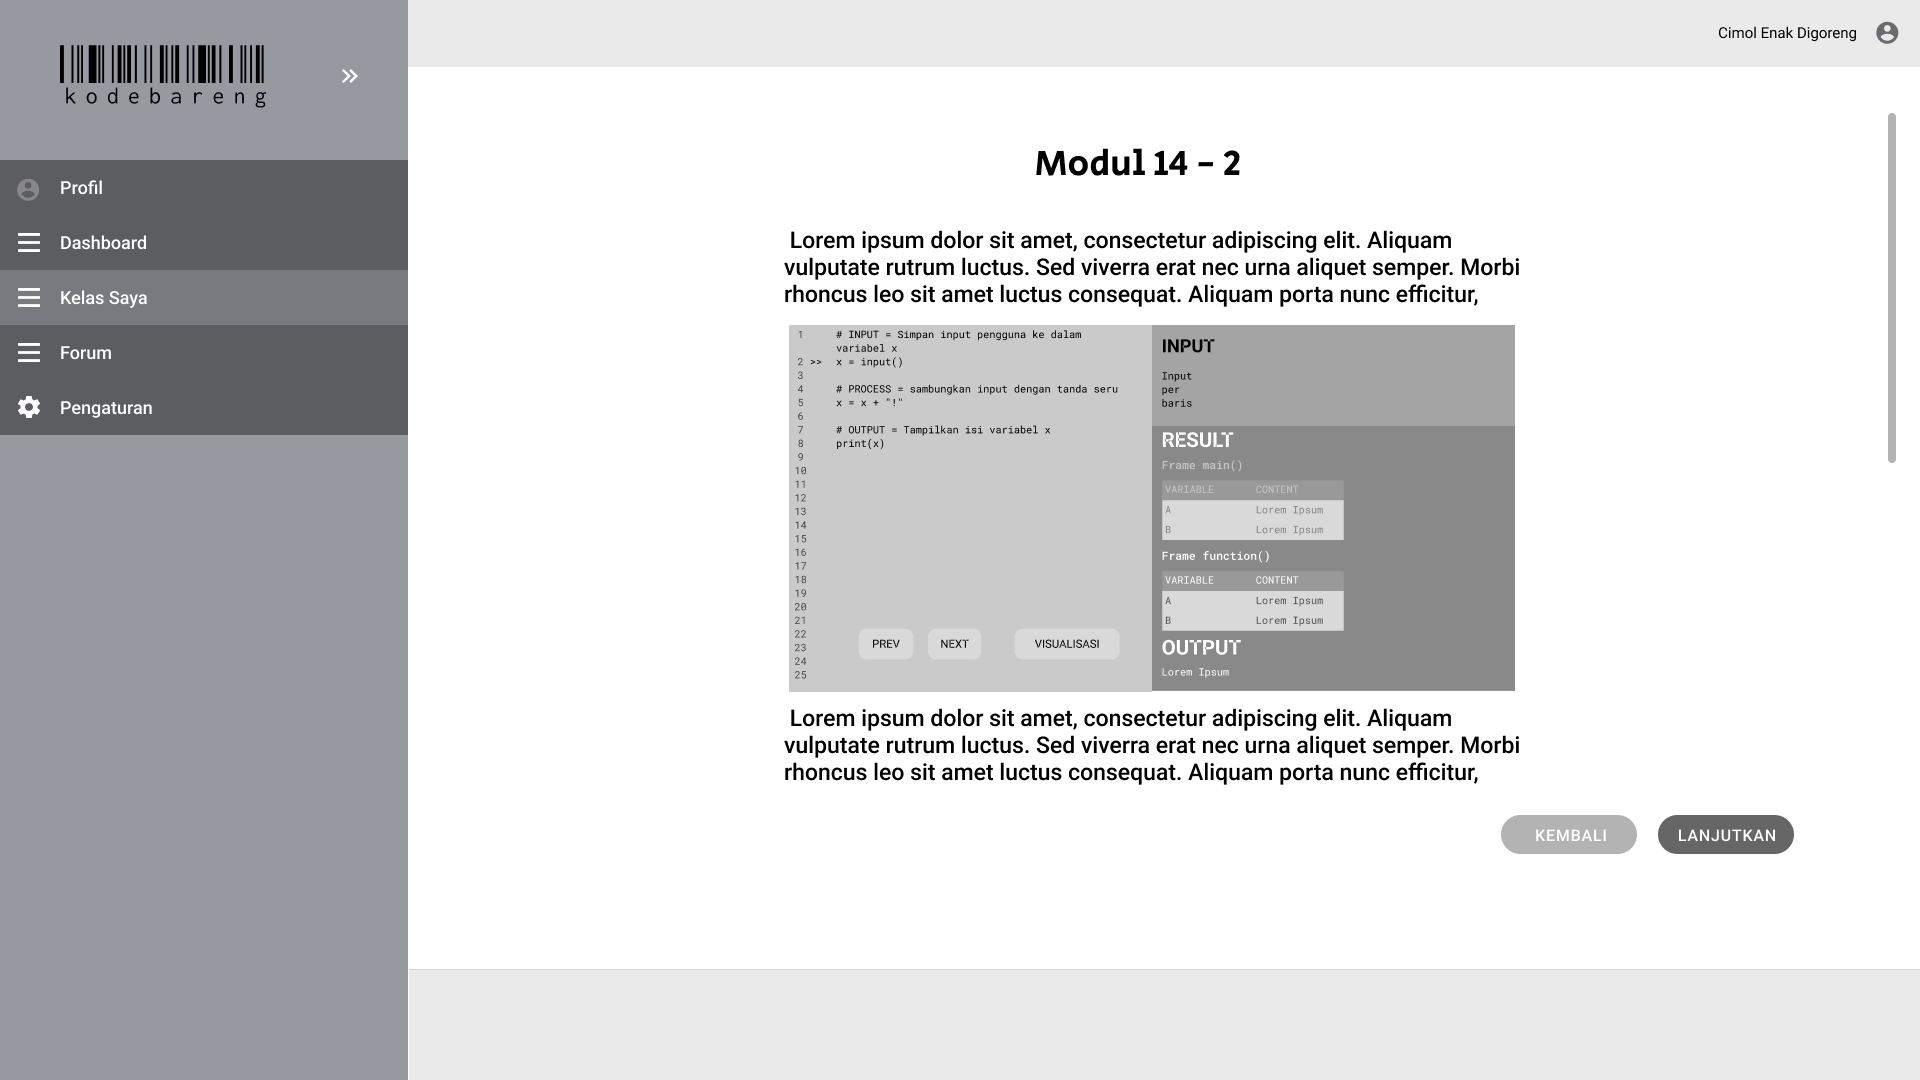
\includegraphics[width=\textwidth]{chapter3/visualizer-explanation.png}
  \caption{Wireframe Visualizer pada Explanation Stage \\ Sumber: Penulis (2022)} \label{fig:wireframe-explanation}
\end{figure}

\begin{figure}[H]
  \centering
  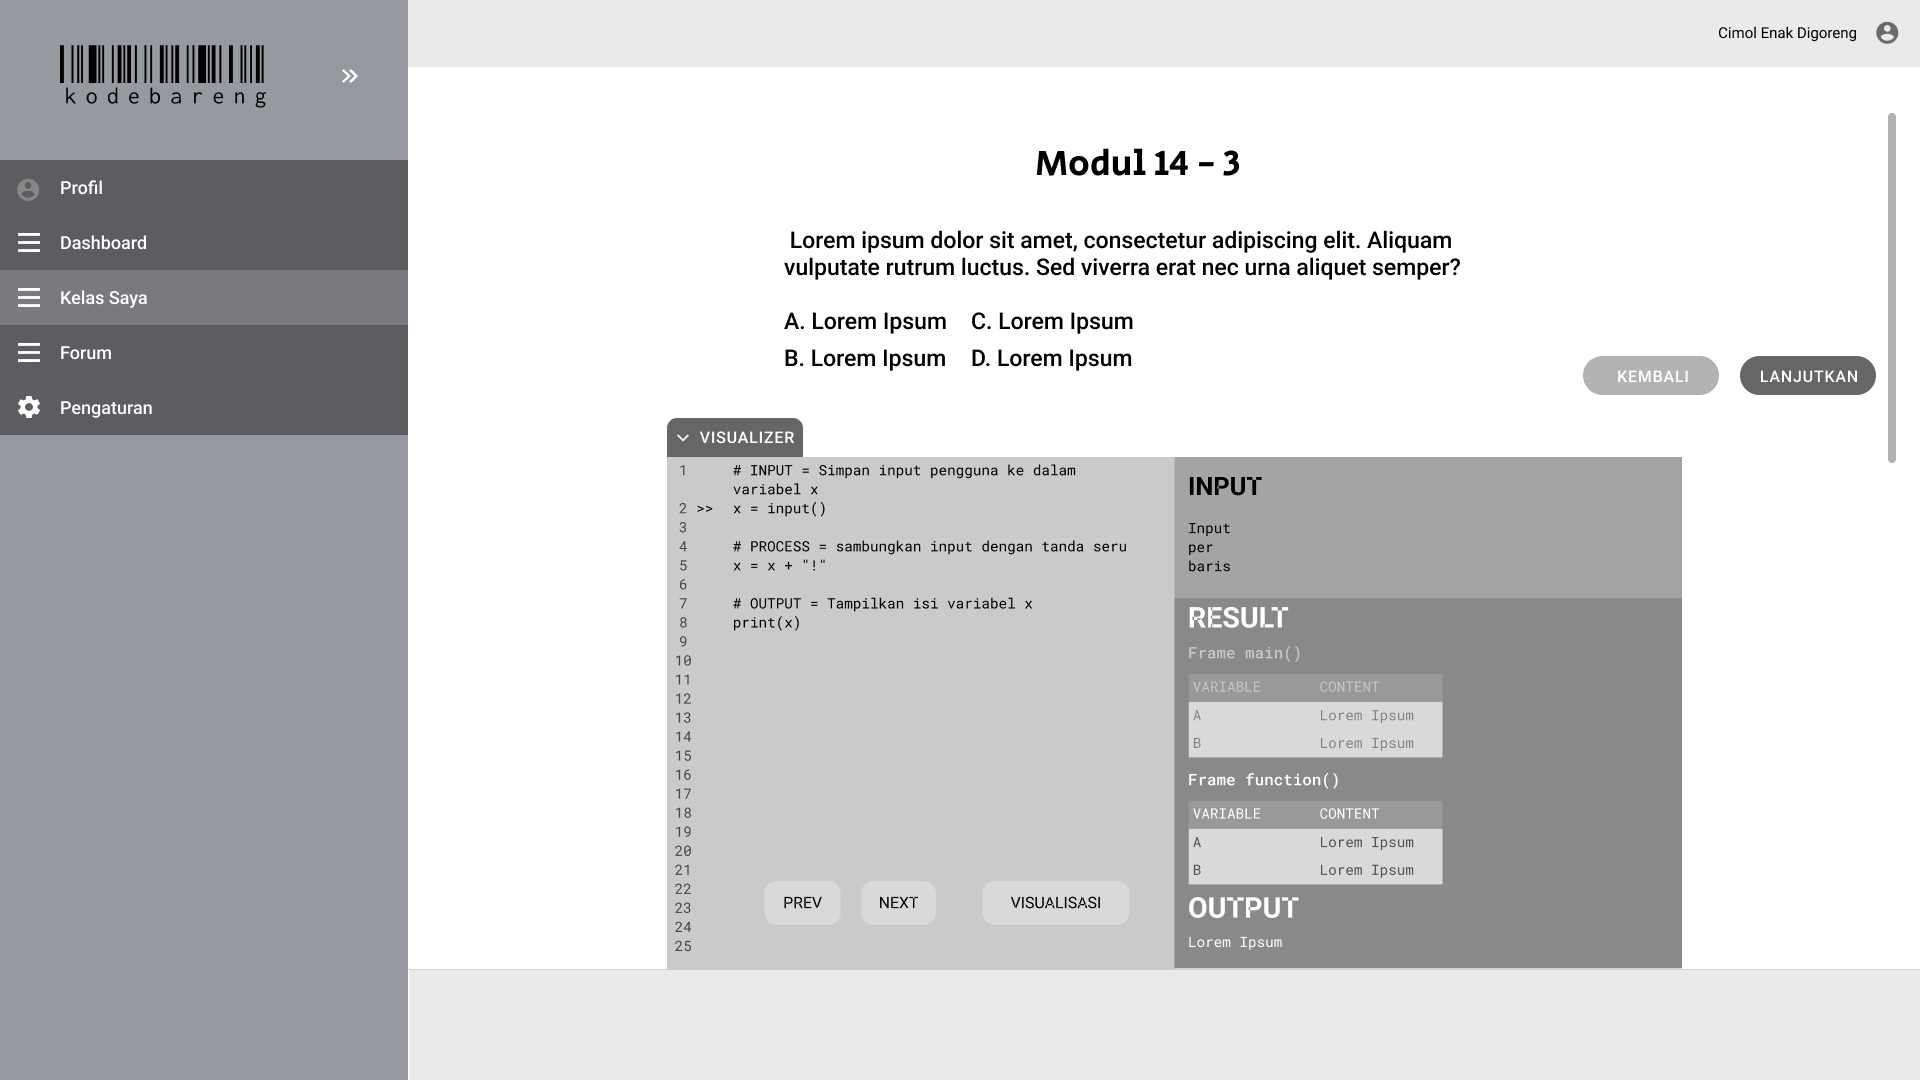
\includegraphics[width=\textwidth]{chapter3/visualizer-quiz.png}
  \caption{Wireframe Visualizer pada Quiz Stage \\ Sumber: Penulis (2022)} \label{fig:wireframe-quiz}
\end{figure}

\begin{figure}[H]
  \centering
  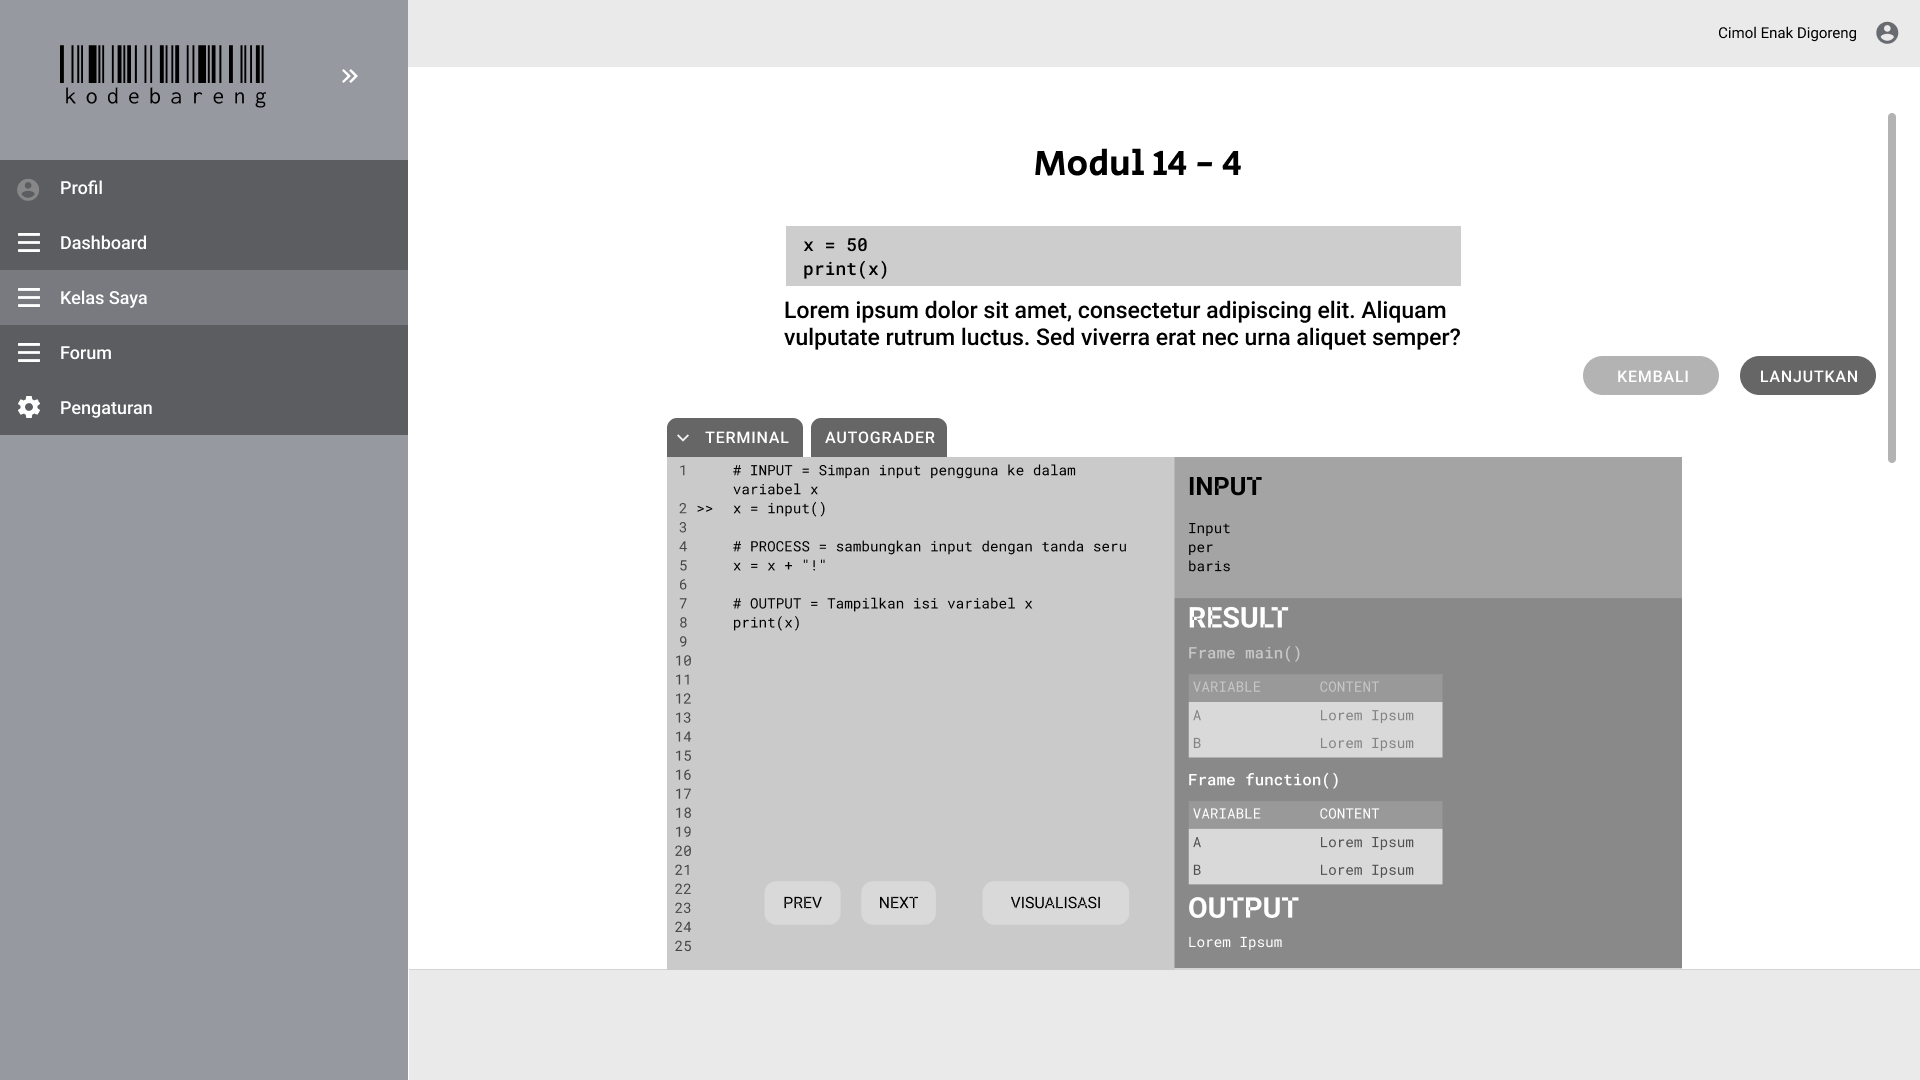
\includegraphics[width=\textwidth]{chapter3/visualizer-lesson.png}
  \caption{Wireframe Visualizer pada Lesson Stage \\ Sumber: Penulis (2022)} \label{fig:wireframe-lesson}
\end{figure}

Pada sistem \textit{Backend}, ditambahkan rute baru pada \textit{Stage Controller} untuk dapat mengolah permintaan visualisasi eksekusi kode. Dibuat juga fungsi-fungsi \textit{Helper} tambahan untuk mengolah permintaan tersebut dan melanjutkannya pada sistem eksekutor apabila kode diperbolehkan untuk dieksekusi.

Pada sistem \textit{Executor}, dibuat komponen-komponen baru untuk mendapatkan informasi yang dibutuhkan untuk visualisasi. Komponen \verb|PDB (debugger)| merupakan komponen bawaan \verb|Python| yang dapat digunakan untuk melakukan \textit{debugging} pada suatu kode. Komponen \verb|Executor| digunakan untuk mengeksekusi kode program menggunakan PDB sehingga dapat dengan otomatis menjelajahi eksekusi kode program dan mendapatkan \textit{stack trace}. Komponen \verb|Parser| digunakan untuk mengolah hasil eksekusi serta \textit{stack trace} dari \verb|Executor| sehingga dapat dimanfaatkan untuk visualisasi eksekusi kode. Terdapat juga modifikasi pada Kontroller dan Autograder agar dapat menyesuaikan dengan spesifikasi kebutuhan fungsional. Rancangan alur kerja komponen Executor dan Parser dapat dilihat pada \autoref{fig:activity-executor}

\begin{figure}[H]
  \centering
  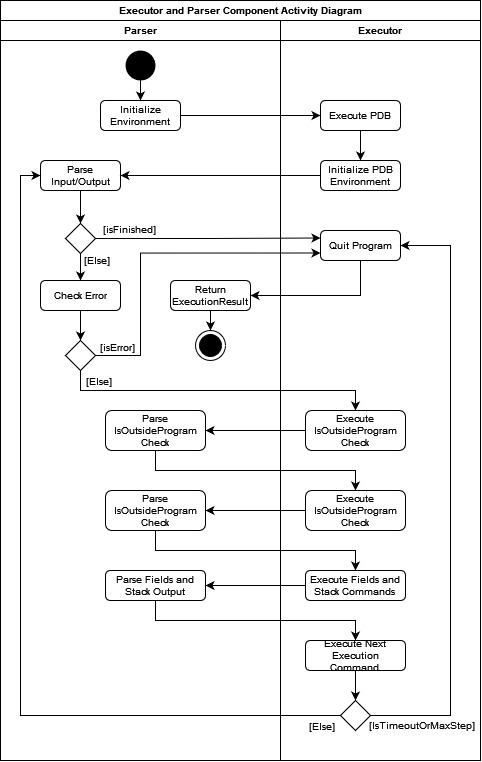
\includegraphics[width=0.8\textwidth]{chapter3/activity-executor.jpg}
  \caption{Activity Diagram Komponen Executor dan Parser \\ Sumber: Penulis (2022)} \label{fig:activity-executor}
\end{figure}